% !TeX document-id = {2e1841e8-ce56-4d5c-95b9-f6ac1d5fc83f}
% !TeX TXS-program:compile = txs:///pdflatex/[--shell-escape]
%\RequirePackage{fix-cm}
\documentclass[border={-1.1mm -1.1mm -3mm -1mm}]{standalone}
\usepackage[utf8]{inputenc}
\usepackage{lmodern}
\usepackage{graphics}
\usepackage{tikz,filecontents, pgfplots}
\pgfplotsset{compat=1.5}
\usepackage{siunitx}
\usepackage{textcomp}
\usepackage{gensymb}
\usepackage{pgfplots}
\usetikzlibrary{positioning,spy}
\usepackage{amsmath}
\usetikzlibrary{decorations,decorations.markings,decorations.text}
\usetikzlibrary{arrows,
	arrows.meta,
	decorations.pathmorphing,
	calc,%
	decorations.pathmorphing,%
	decorations.markings,
	fadings,%
	shadings,%
	positioning,
	spy,
	shapes,
	shapes.geometric,
	shapes.arrows,
	fit,
	plotmarks,}
\usetikzlibrary{arrows}



\usepackage{tikz-dimline}


\tikzset{
	%box/.style  = {draw,rectangle, minimum width=5cm, minimum height=1.2cm, text centered, text width=5cm, font=\Large},
	myarrow/.style = {line width=40mm, draw=blue, -triangle 60, }
}
\begin{document}
\begin{tikzpicture}[spy using outlines={circle,red,every spy on node/.append style={line width=0.1mm},connect spies}]


\node[anchor=south](ga1) at (current page.south) {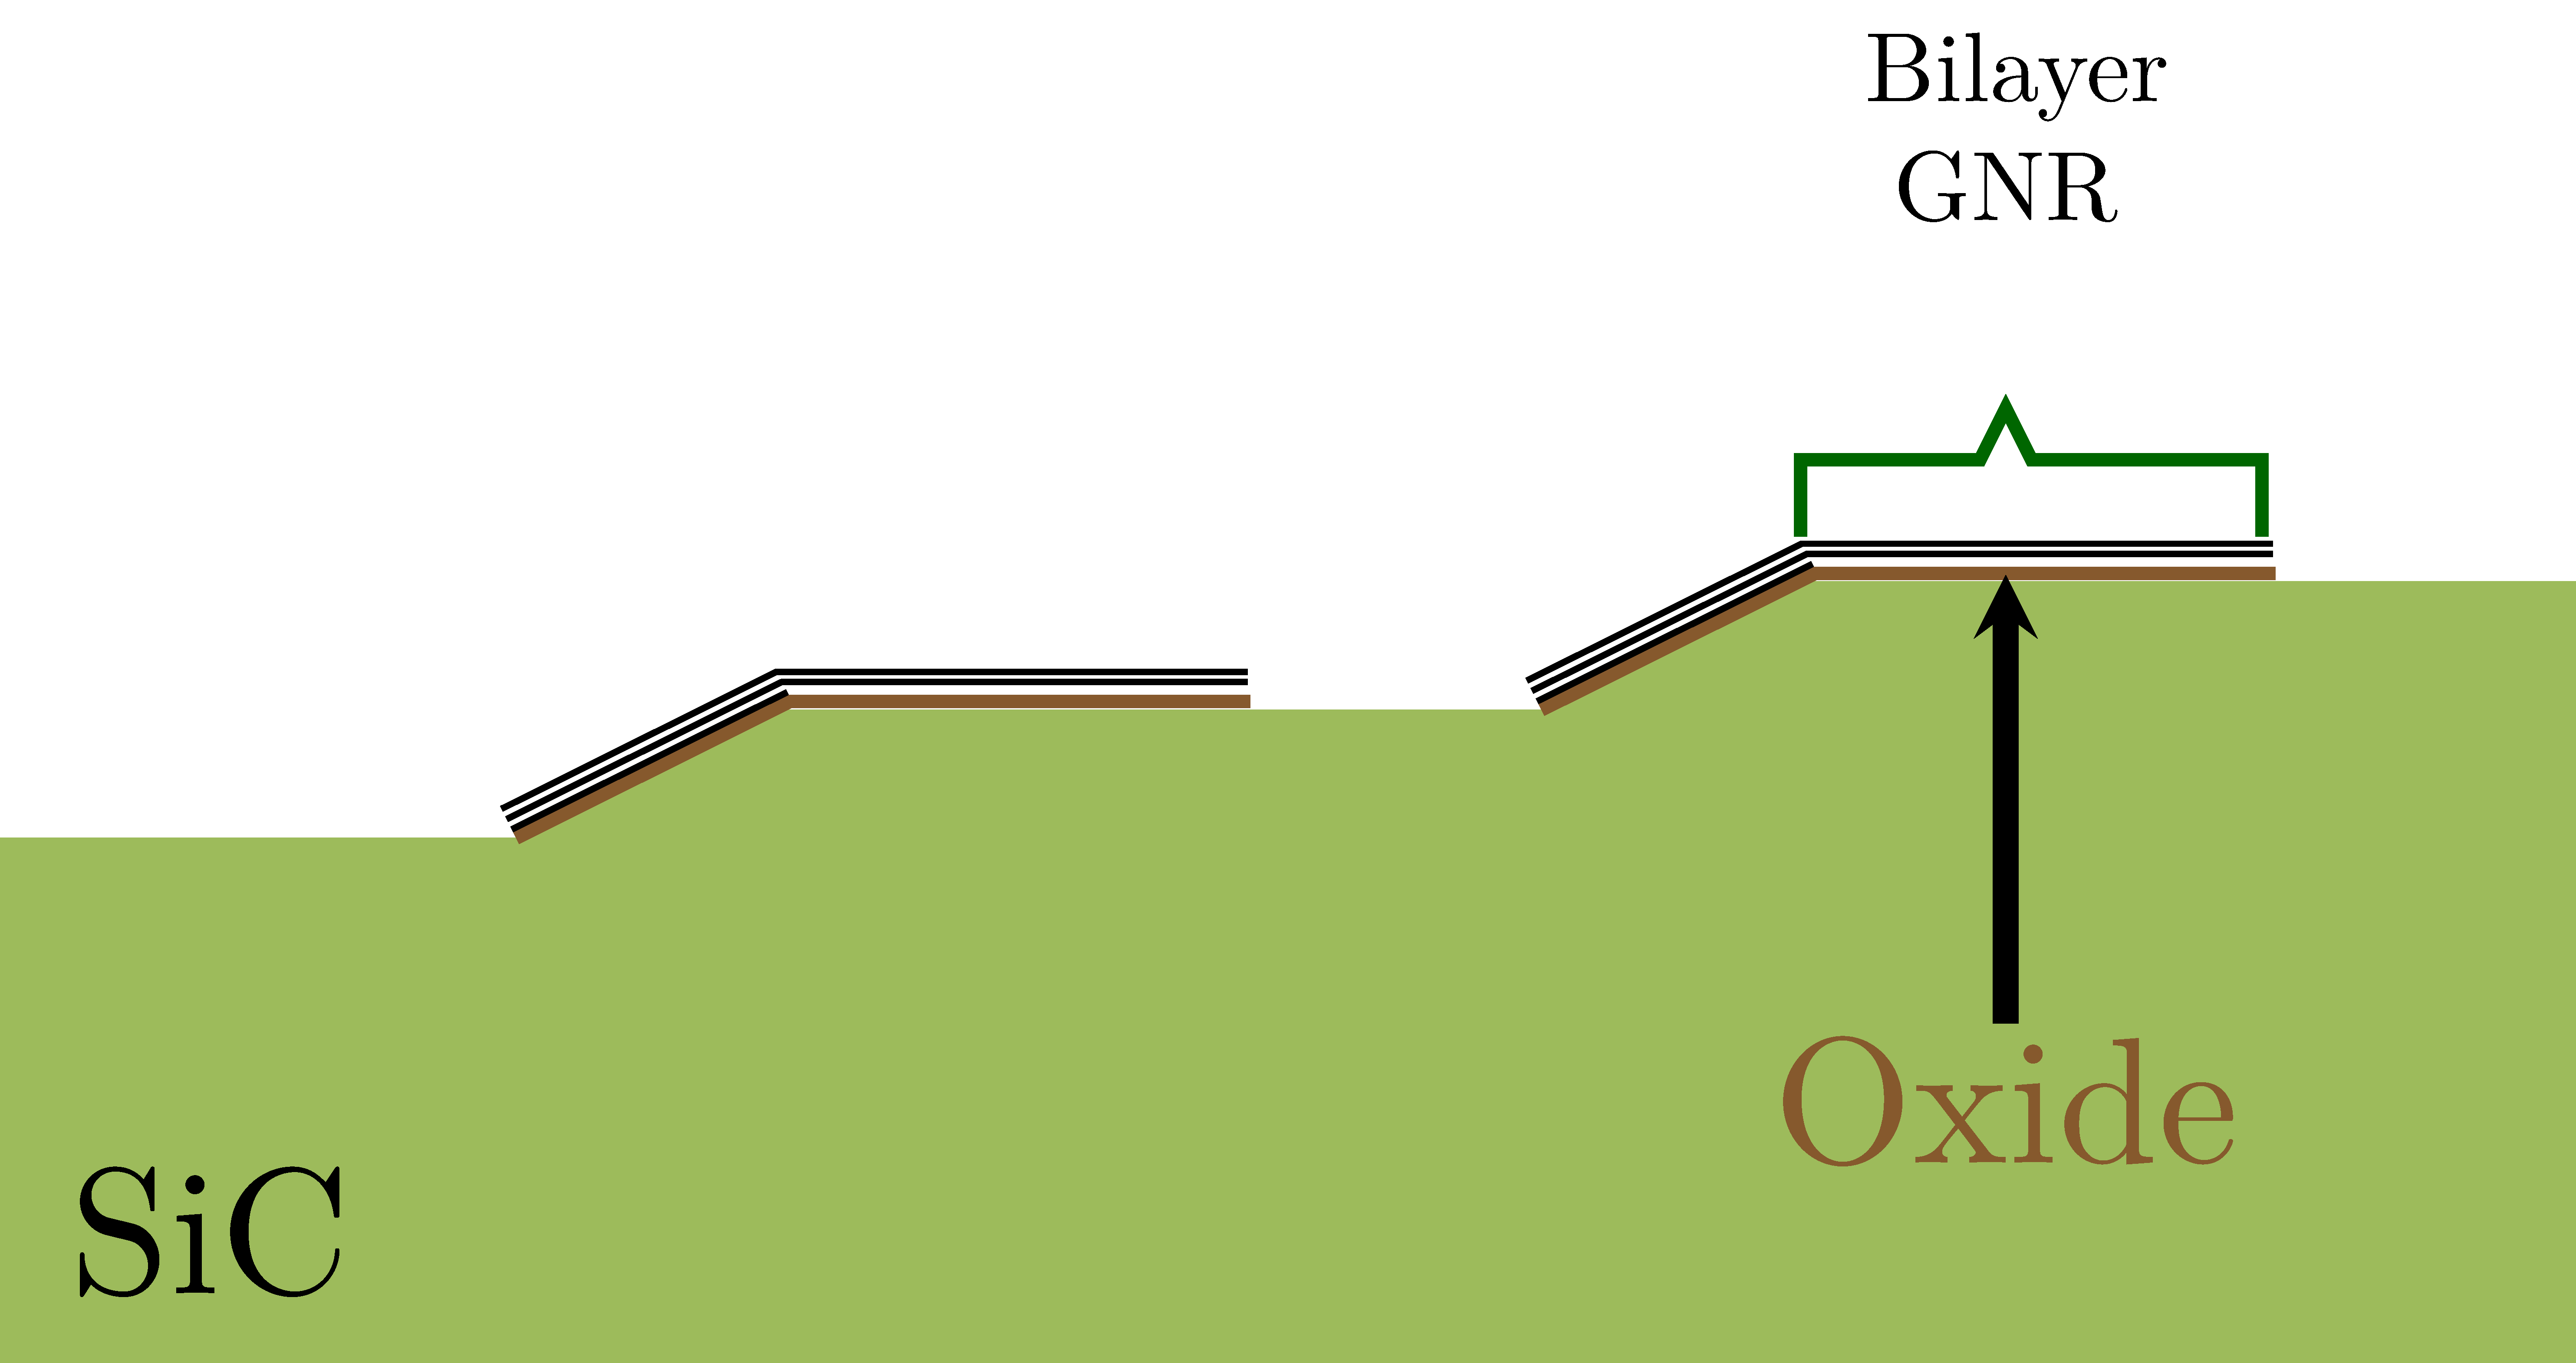
\includegraphics[scale=0.25]{GA}};
\node[anchor=south west,xshift=-45mm,yshift=-0mm](nsom1) at (ga1.center) {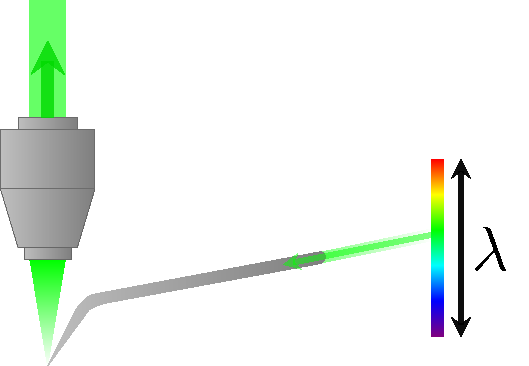
\includegraphics[scale=2]{GA-2}};

%\node[anchor=south east,xshift=-10mm,yshift=5mm,draw,inner sep=0mm](nsom2) at (ga1.south west){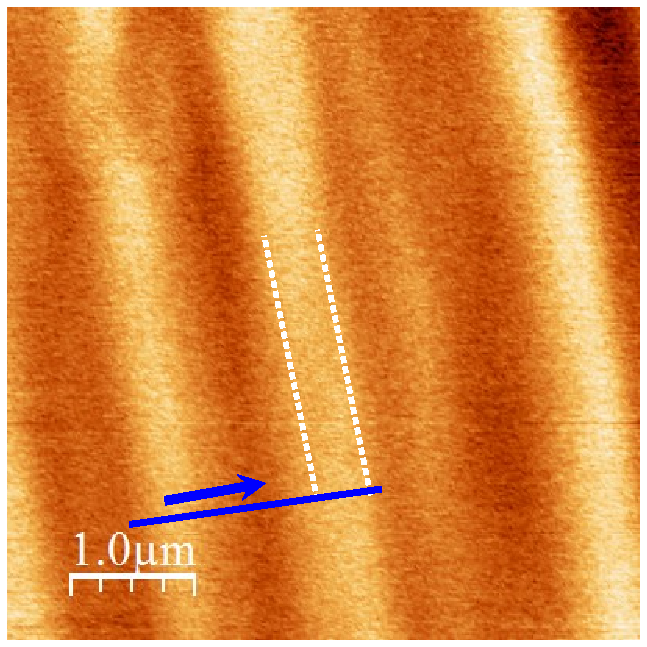
\includegraphics[scale=0.145]{GA-3}};
%\node[anchor=south,xshift=-1.56mm,yshift=7mm](nsom3) at (nsom2.center) {\includegraphics[scale=0.8]{spectra}};
%\node[anchor=west,xshift=0mm,xshift=2.5cm,yshift=0cm](nsom4) at (nsom3.east) {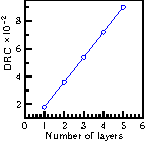
\includegraphics[scale=0.8]{DRC}};
%\draw[-{stealth},line width=10mm] (nsom2.center)--([xshift=80mm]nsom3.center);
%\node[circle, minimum width=90mm,draw,anchor=center,line width=3mm](foc1) at ([xshift=-0.5cm,yshift=-5cm]nsom2.center){};

%\draw [myarrow,opacity=1] (nsom2.north) -- ([yshift=400mm,xshift=90mm]nsom3.south);
%\node[draw, single arrow,red,
%minimum height=80cm, minimum width=150mm,
%single arrow head extend=1mm,
%fill=red,
%opacity=0.2,
%xshift=-1cm,
%anchor=west, rotate=90] at (nsom2.center) {};
%\node[draw, 
%single arrow,
%red,
%minimum height=70cm, minimum width=150mm,
%single arrow head extend=1mm,
%yshift=20cm,
%fill=red,
%opacity=0.2,
%anchor=west, rotate=0] at (nsom3.east) {};

%\draw[line width=3mm] ([xshift=0mm]nsom2.south west)--(foc1.south);
%\draw[line width=3mm] ([xshift=0mm]nsom1.south west)--(foc1.north east);
\coordinate (region1) at ([xshift=7cm,yshift=1cm]ga1.center);
\coordinate (pos1) at (15.5cm,13.75cm);
%
\spy [size=6cm,
magnification=5,
every spy in node/.append style={line width=0.1mm},
spy connection path=
{\draw[densely dashed,red,line width=0.1mm] (tikzspyonnode.east) -- (tikzspyinnode.east);
	\draw[dashed,red,line width=0.1mm] (tikzspyonnode.west) -- (tikzspyinnode.west);},
]  on (region1) in node[fill=white] at (pos1) ;    


\end{tikzpicture}

\end{document}